% !TEX root = ../bachlor-arbeit.tex
Before starting to implement the Algorithm, we need to define which metasurface stacks the it is allowed to produce. This was already partly motivated in the introduction: We want easy to manufacture metasurfaces which can produce a high variety of transmission spectra when stacked.
Physically, we consider stacks which are homogeneously illuminated by plane waves and produce transmission spectra $I = I(\lambda) \in [0,1]$.
We are going to use the homogeneous plasmonic metasurfaces discussed in section \ref{sec:plasmonic}. These surfaces can be manufactured via electron beam lithography.
\\

\indent
We want to enable the algorithm to produce custom polarizers. This means we need to be able to control the $x$ and $y$ polarizations separately. 
As shown in section \ref{sec:SASA} paragraph \hyperref[sec:symmetries]{Symmetries}, we cannot use meta-atoms of $C_4$ symmetry for this task. The next simplest geometry is the rectangle. Another limitation given by the manufacturing process is the number of metasurface layers in a stack. Stacks with more than two layers become increasingly hard to manufacture this is why we are going to limit the algorithm to two-layer stacks even though theoretically arbitrary stacks could be used.
\\

\indent
To reach the greatest variety of transmission spectra, we will have to expand the possible geometries slightly. As described in section \ref{sec:plasmonic}, rectangular metaatoms tend to produce a minima in the transmission at a wavelength where incident photons can couple efficiently into SPP's. However, many transmission spectra contain both minima and maxima and at this point we are not able to produce the maxima.
For this reason, we will expand the possible geometries to rectangular holes as seen in the bottom layer of figure \ref{fig:al:two_layers}. This type of metaatom has a low transmission for most wavelengths and only the photons which would have fit the resonance condition of the hole geometry can transmit freely. In a sense, the rectangular hole acts as an inverse to the rectangle in the type of transmission spectra they produce.


\begin{figure}[H]
    \centering
    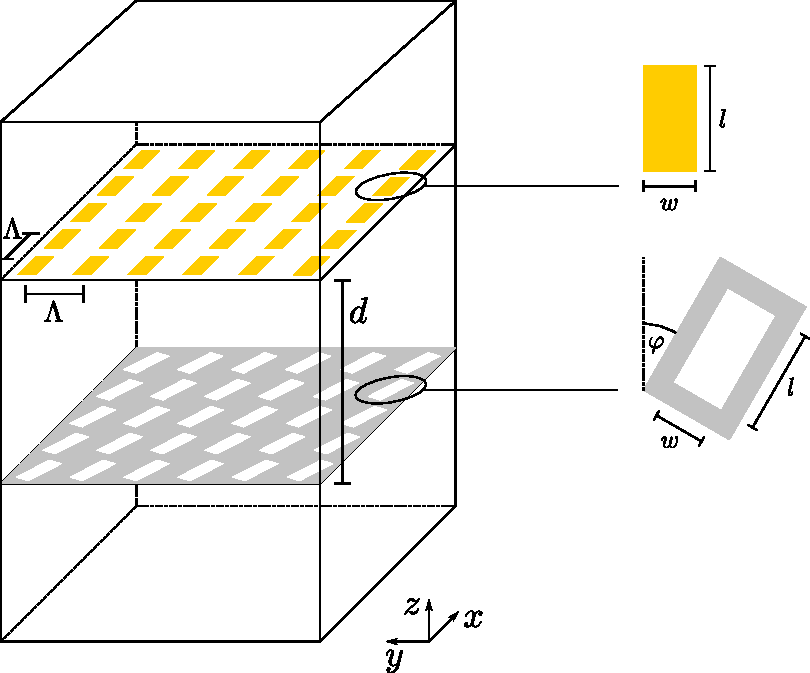
\includegraphics[width=.69\linewidth]{al_two_layers}
    \caption{Schematic of a two layer metasurface stack to visualize all the design parameters
    $\mc D$ which can be set by the algorithm. These include stack parameters $\mc S$ and two sets of layer parameters $\mc L_1$ and $\mc L_2$.
    So ${\mc D = (\mc S, \mc L_1, \mc L_2)}$. The stack parameters consist of the distance between the metasurfaces $d$ and their rotation angle $\varphi$ so $\mc S = (d, \varphi)$. The layer parameters are the width $w$, length $l$ and thickness $t$ of the meta-atom, the period of meta-atoms $\Lambda$ the  material of the layer $m$ and the kind of geometry $g$. So $\mc L = (w,l,t,\Lambda,m,g)$. All of the parameters are continuous except for the choice about the material and geometry.}
    \label{fig:al:two_layers}
\end{figure}


As for the material, we are going to limit the algorithm to Aluminum and Gold. Here we have to remember that every material we add multiplies the amount of metasurfaces which have to be simulated in preparation which is often referred to as the \textit{curse of dimensionality}. This is because more materials are only useful when the corresponding parameter space is sufficiently dense. This ends the design considerations, a visualization of all parameters and the notation we are going to use can be found in figure \ref{fig:al:two_layers}.
